\documentclass[aps,prb,10pt,superscriptaddress,notitlepage]{revtex4-1}
\usepackage{amsmath}

\usepackage{graphicx}
\graphicspath{{figures/}{./}}
\usepackage[caption=false]{subfig}

\setcounter{topnumber}{3}
\setcounter{bottomnumber}{3}
\setcounter{totalnumber}{3}

\usepackage[colorlinks=true, linkcolor=blue, citecolor=red]{hyperref}

\pacs{71.35.Cc, 73.20.Mf, 71.15.Mb, 71.20.Mq, 71.10.-w}

\begin{document}

\title{Supplemental Material for
\emph{Plasmon dispersion in Graphite: A comparison of current \emph{ab initio}
methods}}
\author{Sean M. Anderson}%\email{sma@cio.mx}
    \affiliation{Centro de Investigaciones en \'Optica, 
                Le\'on, Guanajuato, M\'exico}
\author{Bernardo S. Mendoza}%\email{bms@cio.mx}
    \affiliation{Centro de Investigaciones en \'Optica, 
                Le\'on, Guanajuato, M\'exico}
\author{Giorgia Fugallo}%\email{giorgia.fugallo@univ-nantes.fr}
    \affiliation{CNRS, UMR 6607, Laboratorie de Thermique et Energie de Nantes
    (LTeN) Polytech'Nantes, Universit\'e de Nantes, Rue Christian Pauc, F-44306
    Nantes Cedex 3, France}
\author{Francesco Sottile}%\email{francesco.sottile@polytechnique.fr}
    \affiliation{Laboratoire des Solides Irradi\'es, \'Ecole Polytechnique, 
    CNRS, CEA, Université Paris-Saclay, F-91128 Palaiseau, France }
    \affiliation{European Theoretical Spectroscopy Facility (ETSF)}
\date{\today}

\maketitle

%%%%%%%%%%%%%%%%%%%%%%%%%%%%%%%%%%%%%%%%%%%%%%%%%%%%%%%%%%%%%%%%%%%%%%%%%%%%%%%%
%%%%%%%%%%%%%%%%%%%%%%%%%%%%%%%%%%%%%%%%%%%%%%%%%%%%%%%%%%%%%%%%%%%%%%%%%%%%%%%%

\section{The \texorpdfstring{$\pi + \sigma$}{pi + sigma} Plasmon}

Our theoretical calculations do not have to be limited to only the low energy
range used in the experiments. The $\pi + \sigma$ plasmon that occurs in the 20
to 40 eV range retains its plasmonic character for momentum values up to $q
\approx 1.5$ \r{A}$^{-1}$. Figs. \ref{fig:gm-heatmap_hi} and
\ref{fig:gk-heatmap_hi} depict the $q$-dependent dispersion in the 15 to 45 eV
energy range for each calculated method, along the $\Gamma \rightarrow
\mathrm{M}_{4}$ and $\Gamma \rightarrow \mathrm{K}_{4}$ paths, respectively. One
crucial remark about these results concerns the number of bands included in each
calculation; with the exception of the BSE CP calculation, all methods include
80 total bands in order to obtain well-converged results over the full energy
range. The BSE CP calculation, due to the considerable computational expense of
diagonalizing the complete Hamiltonian, only includes 20 total bands which is
enough to obtain convergence for the low energy range of the $\pi$ plasmon, but
not enough for the high energy range presented here. Therefore, this data cannot
be used for quantitative analysis, although the general trend can be readily
visualized.

Available experimental data \cite{zeppenfeldZP71, buchnerPSSB77,
marinopoulosPRB04} shows that the $\pi + \sigma$ plasmon peak, for $q = 0$
\r{A}$^{-1}$, is between 25 to 30 eV. As the value of $q$ increases, the peak
widens, decreases slightly in intensity, and moves towards higher energies. We
find that this behavior is well reproduced with methods that include the
coupling terms in the excitonic Hamiltonian, and our calculations predict that
this plasmon continues to increase in width and decrease in intensity until
almost fully dissipating at large values of $q$. The BSE CP calculation, as
mentioned above, does not have enough bands included in order to reproduce the
fine features and intensity of the peak. However, the general trend is the same.
On the other hand, methods that use the Tamm-Dancoff approximation and neglect
these coupling terms tell a different story altogether. These methods tend to
substantially overestimate the peak energy position for low values of $q$, have
an intensity that is several times larger than the experimental value, that very
rapidly diminishes in intensity towards
medium values of $q$. This behavior does not fit the aforementioned experimental
data at all. The dispersive behavior of the $\pi + \sigma$ plasmon is very
similar for both the $\Gamma \rightarrow \mathrm{M}_{4}$ and $\Gamma \rightarrow
\mathrm{K}_{4}$ paths.

\begin{figure}[t]
\centering
\subfloat[$q$ values along the $\Gamma \rightarrow \mathrm{M}_{4}$ path.
\label{fig:gm-heatmap_hi}]
{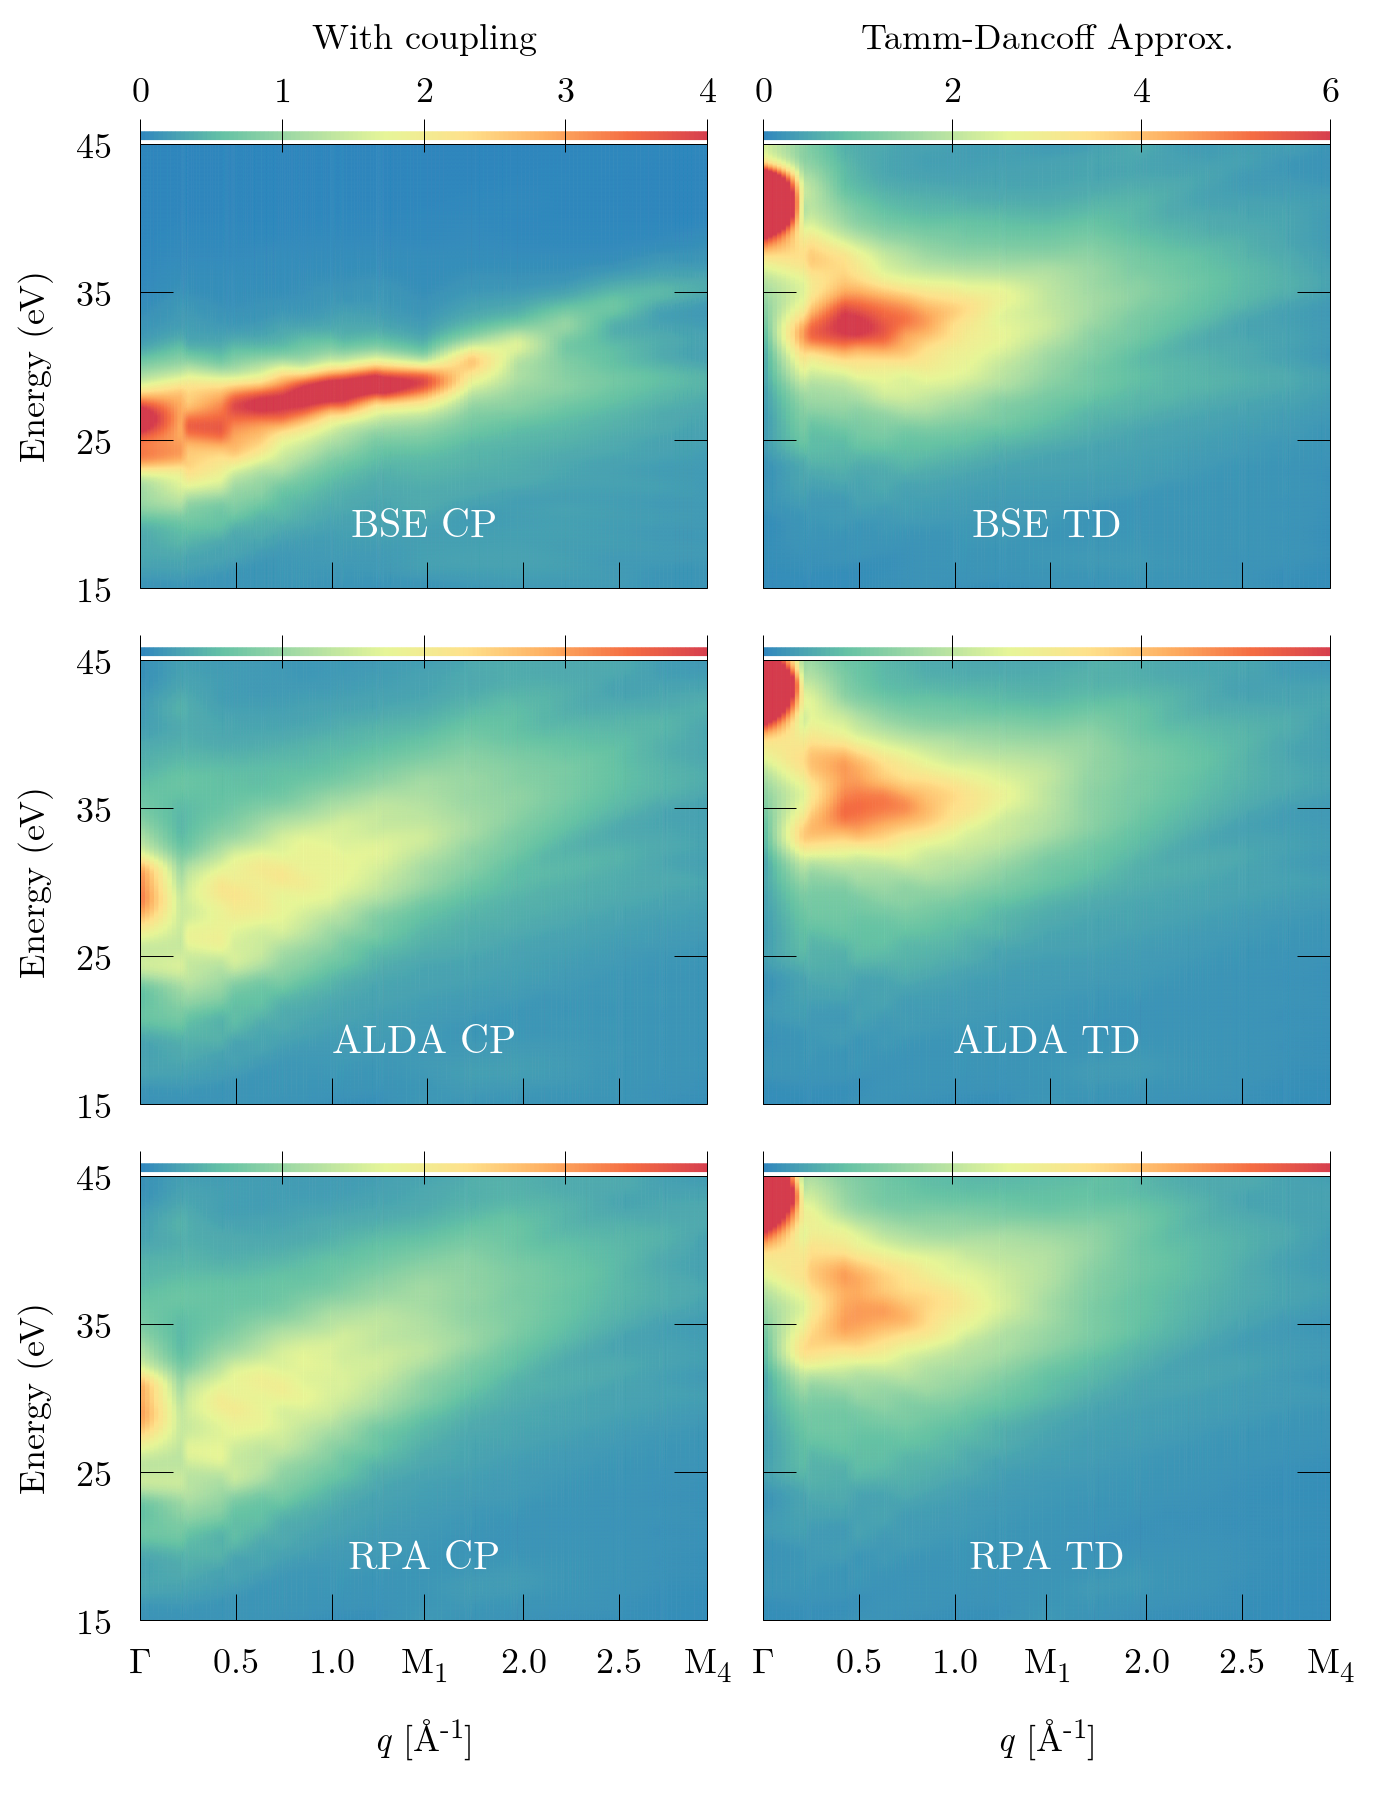
\includegraphics[width=0.45\linewidth]{sup-fig01a}}
\hfill
\subfloat[$q$ values along the $\Gamma \rightarrow \mathrm{K}_{4}$ path.
\label{fig:gk-heatmap_hi}]
{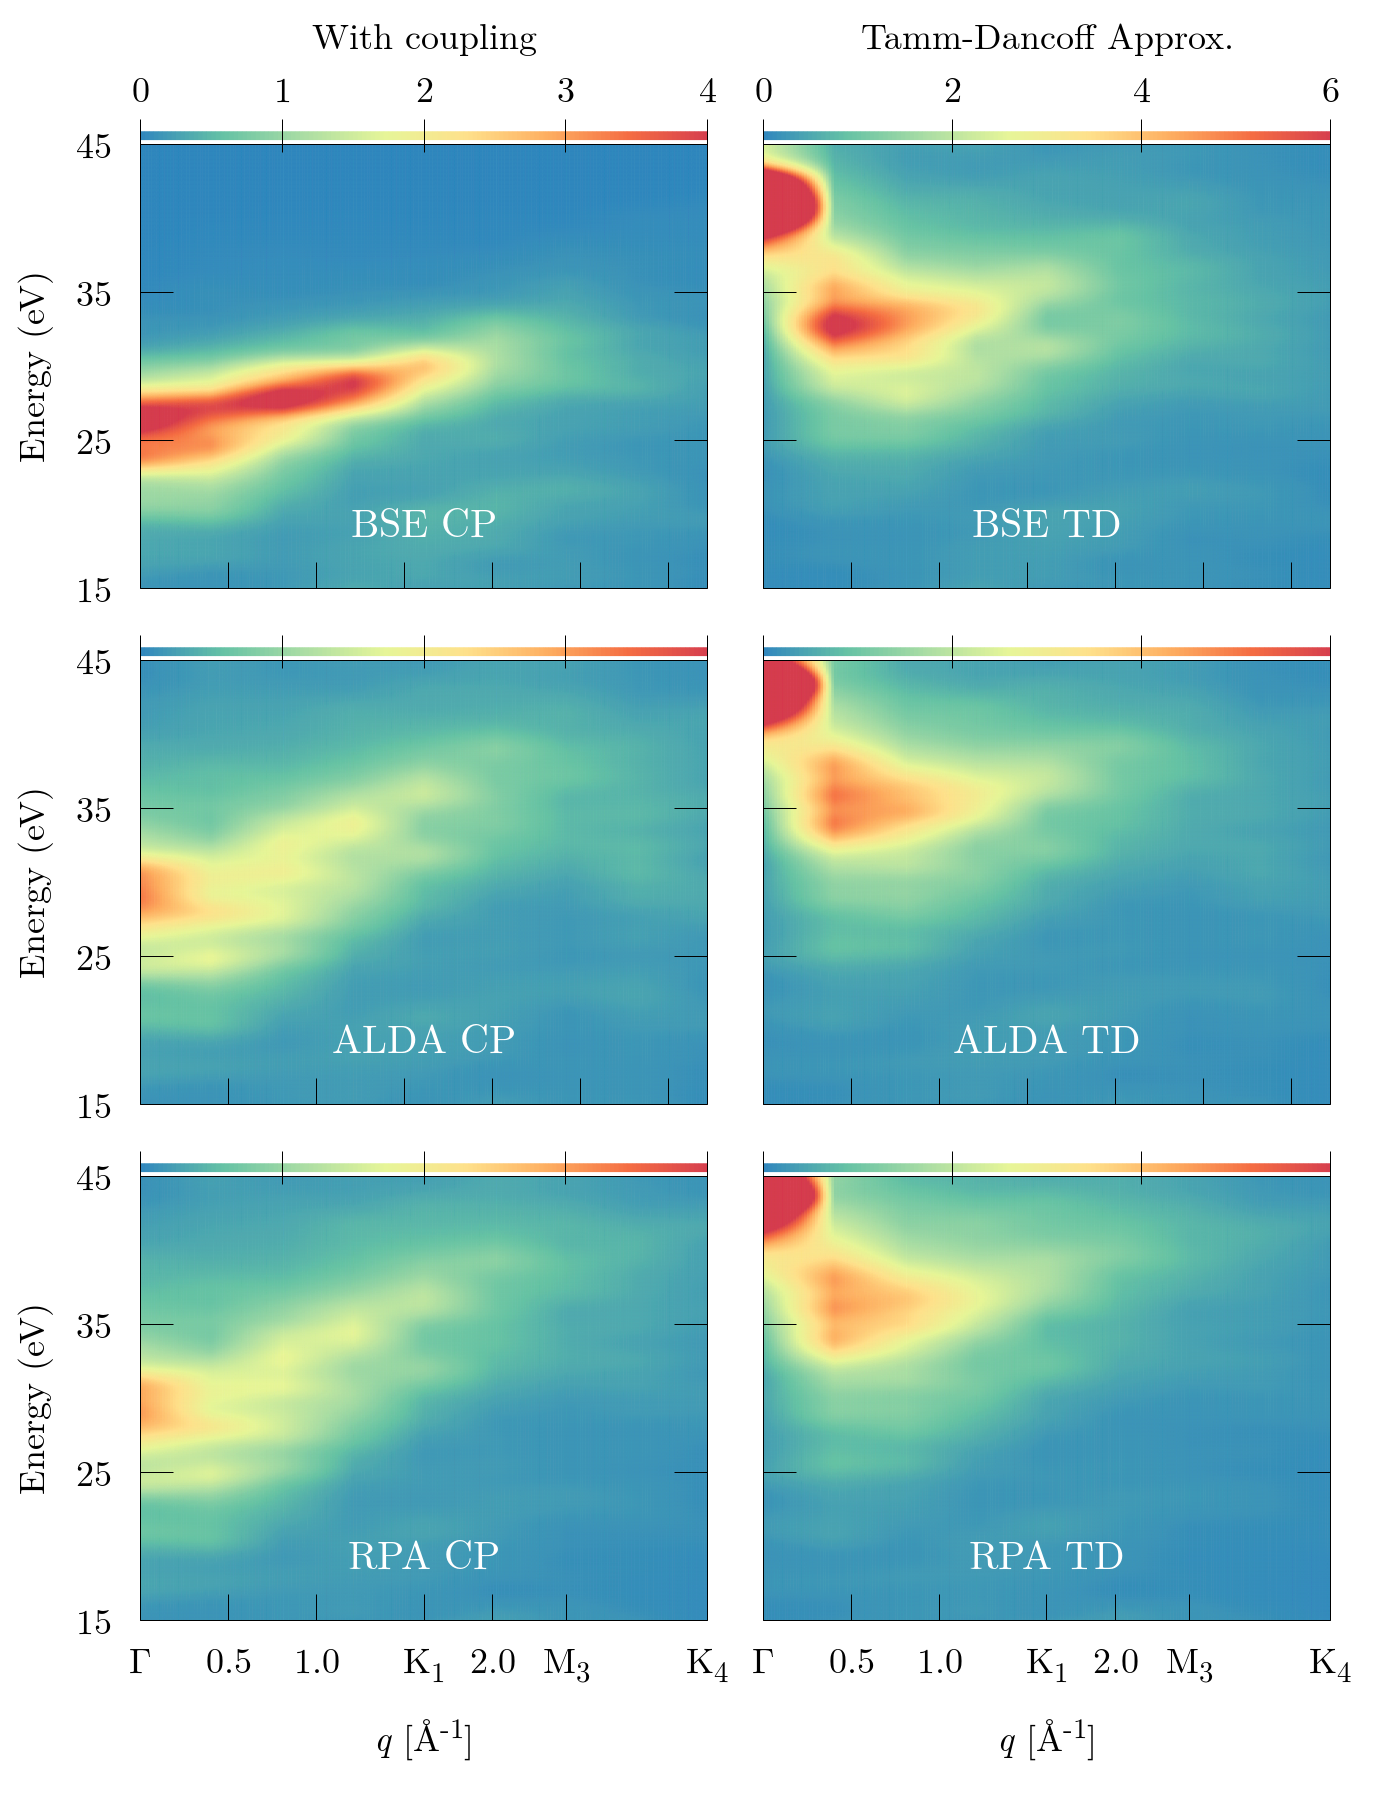
\includegraphics[width=0.45\linewidth]{sup-fig01b}}
\caption{Color map representations of the calculated EEL spectra vs. transfered
momentum ($q$) for the $\pi + \sigma$ plasmon region. Methods including the
coupling terms in the excitonic Hamiltonian are shown in the left column, and
methods neglecting these terms (Tamm-Dancoff approximation) are shown in the
right column. The EEL intensity is represented by the color palette ranging from
blue to red.}
\label{fig:heatmaps}
\end{figure}

These plots mark a striking visual difference between using the full excitonic
Hamiltonian and the TDA; the latter is simply not well-suited for describing
the $\pi + \sigma$ plasmon. Overall, methods that include the coupling terms
offer the best agreement with experiment;
The BSE can accurately describe both exciton and plasmon excitations when used with
the full Hamiltonian as the coupling terms are crucial for accurately describing
the plasmon behavior.

%%%%%%%%%%%%%%%%%%%%%%%%%%%%%%%%%%%%%%%%%%%%%%%%%%%%%%%%%%%%%%%%%%%%%%%%%%%%%%%%
%%%%%%%%%%%%%%%%%%%%%%%%%%%%%%%%%%%%%%%%%%%%%%%%%%%%%%%%%%%%%%%%%%%%%%%%%%%%%%%%

\section{Benchmarks}\label{sec:bench}

During the course of this study, we were able to gather a significant amount of
real-world performance data for the purpose of benchmarking the different
calculations. Table \ref{tab:times} presents the most general time metrics for
each of the different methods featured in this work; these values include the
entire calculation time, from reading the input files to writing the final
datasets. The standard deviation ($\sigma$) for each value was determined from
the multiple calculations required for each grid of \textbf{k}-points. In
general, $\sigma$ merely represents the normal fluctuations in clock speed and
available resources that occur in any computing system. The compute nodes used
in these benchamarks consist of three Intel Xeon E7-8860v3 platforms with clock
speeds of 2.20 GHz. Each node has four processors for a total of 64 cores and 3
TB of DDR4 RAM memory.

These benchmarks make it clear that solving the BSE the full excitonic
Hamiltonian implies an enormous leap in computational time; for this particular
grid, the time is up to 5 orders of magnitude larger. Fortunately, this time can
be greatly reduced by further parallelizing the number of \textbf{k}-points over
more cores. As mentioned above, each of our compute nodes has 64 cores allowing
us to parallelize over 192 cores total. Table \ref{tab:cores} presents the
duration (in days) of the full excitonic calculation for the
14$\times$14$\times$02 grid as a function of the number of cores. The total time
is reduced by around 50\% by doubling the number of cores from 64 to 128 (at
which point we more or less reach the scalability range of our code). This study
is obviously not exhaustive as the number of cores used was not optimal; the
14$\times$14$\times$02 has 392 \textbf{k}-points which is not evenly divisible
by 64, 128, or 192. However, we can clearly see that the parallelization is
still very effective across two nodes, probably reaching peak efficiency at 98
cores with 4 \textbf{k}-points per core. However, as these numbers were obtained
over the course of many trials and for such long calculations, emphasis was
given on the number of simultaneous calculations possible rather than the most
optimized parallelization for each one.

Lastly, the full excitonic calculation also has significant memory requirements
that must be taken into consideration. The memory required for storing the
excitonic Hamiltonian (in GB) can be calculated using the following expression,
\begin{equation}\label{eq:mem}
(k_{x}\times k_{y}\times k_{z}\times N_{v}\times N_{c})^{2} \times
\frac{8\, \mathrm{bytes}}{1024^{3}},
\end{equation}
where $k_{x}$, $k_{y}$, and $k_{z}$ define the \textbf{k}-point grid, and
$N_{v}$ and $N_{c}$ are the number of valence and conduction bands,
respectively. Fig. \ref{fig:bands} depicts the relation from Eq. \eqref{eq:mem}
(solid red line) using the left-side axis. The size of the excitonic Hamiltonian
was around 300 GB for this work, with 80 total bands included for most
calculations. The blue dots and dotted line are the raw calculation times (in
hours) and the quartic fit for the BSE TD method. The reduced Hamiltonian in the
TDA, coupled with the very efficient Haydock iterative scheme vastly reduces the
calculation time compared to the BSE with the full Hamiltonian. However,
calculation time still increases very rapidly with the number of bands; which is
particularly troublesome for systems with spectral features present at high
energies. Unfortunately, we are not able to provide this same benchmark for the
BSE CP method, as calculation time became unwieldy above 20 total bands.

\begin{figure}[t]
{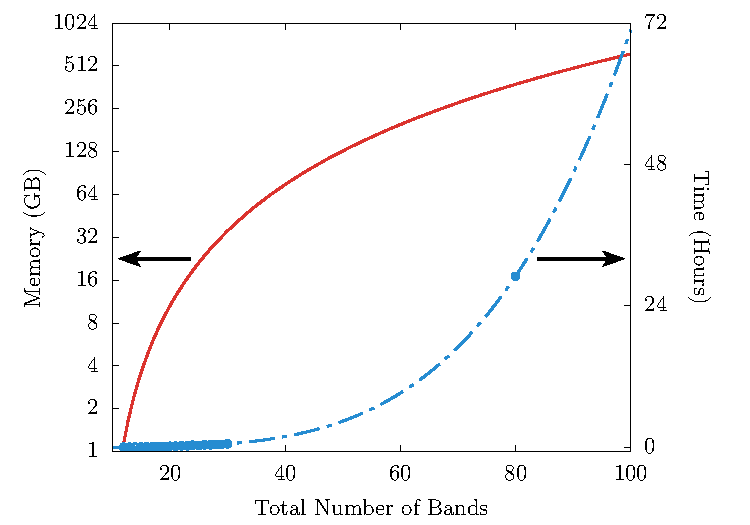
\includegraphics[width=0.5\linewidth]{sup-fig02}}
\caption{Memory usage (in GB) as a function of the total number of
bands (red solid line, left-hand scale), and calculation time as a function of
the total number bands included in the BSE TD method for the 14x14x02
\textbf{k}-point grid, parallelized over 64 cores (blue circles, right-hand
scale). The blue dotted line is a quartic fit, where $f(N) =
7.082\times10^{-7}N^{4}$ in hours.}
\label{fig:bands}
\end{figure}

\begin{table}[t]
\caption{Duration in minutes for each of the different levels of approximation
for the 14$\times$14$\times$02 (392) grid of \textbf{k}-points, alongside the
standard deviation and the number of cores used. A total of 20 bands were
included in the calculation.}
\label{tab:times}
\begin{ruledtabular}
\begin{tabular}{ r c c c c c }
Method & Duration\,(min) & $\sigma$\,(min) & Cores\\
\hline
BSE CP  & 20559.13       & 472.52          & 64\\
BSE TD  &    40.05       &   0.32          & 64\\
ALDA CP &     7.67       &   1.10          & 32\\
ALDA TD &     1.90       &   0.17          & 32\\
RPA CP  &     3.35       &   0.43          & 32\\
RPA TD  &     1.63       &   0.25          & 32
\end{tabular}
\end{ruledtabular}
\end{table}

\begin{table}[t]
\caption{Duration in days for each of the different levels of approximation
for the 14$\times$14$\times$02 (392) grid of \textbf{k}-points, alongside the
standard deviation and the number of cores used. A total of 20 bands were
included in the calculation.}
\label{tab:cores}
\begin{ruledtabular}
\begin{tabular}{ r c c c c }
Cores & Duration\,(Days) & $\sigma$\,(Days) & \textbf{k}-points\\
\hline
 64   & 14.3             & 0.33             & 392 \\
128   &  7.4             & 0.00             & 392 \\
192   &  7.8             & 0.21             & 392
\end{tabular}
\end{ruledtabular}
\end{table}

%%%%%%%%%%%%%%%%%%%%%%%%%%%%%%%%%%%%%%%%%%%%%%%%%%%%%%%%%%%%%%%%%%%%%%%%%%%%%%%%
%%%%%%%%%%%%%%%%%%%%%%%%%%%%%%%%%%%%%%%%%%%%%%%%%%%%%%%%%%%%%%%%%%%%%%%%%%%%%%%%

% \bibliographystyle{apsrev4-1}
% \bibliography{refs}

\begin{thebibliography}{3}%
\makeatletter
\providecommand \@ifxundefined [1]{%
 \@ifx{#1\undefined}
}%
\providecommand \@ifnum [1]{%
 \ifnum #1\expandafter \@firstoftwo
 \else \expandafter \@secondoftwo
 \fi
}%
\providecommand \@ifx [1]{%
 \ifx #1\expandafter \@firstoftwo
 \else \expandafter \@secondoftwo
 \fi
}%
\providecommand \natexlab [1]{#1}%
\providecommand \enquote  [1]{``#1''}%
\providecommand \bibnamefont  [1]{#1}%
\providecommand \bibfnamefont [1]{#1}%
\providecommand \citenamefont [1]{#1}%
\providecommand \href@noop [0]{\@secondoftwo}%
\providecommand \href [0]{\begingroup \@sanitize@url \@href}%
\providecommand \@href[1]{\@@startlink{#1}\@@href}%
\providecommand \@@href[1]{\endgroup#1\@@endlink}%
\providecommand \@sanitize@url [0]{\catcode `\\12\catcode `\$12\catcode
  `\&12\catcode `\#12\catcode `\^12\catcode `\_12\catcode `\%12\relax}%
\providecommand \@@startlink[1]{}%
\providecommand \@@endlink[0]{}%
\providecommand \url  [0]{\begingroup\@sanitize@url \@url }%
\providecommand \@url [1]{\endgroup\@href {#1}{\urlprefix }}%
\providecommand \urlprefix  [0]{URL }%
\providecommand \Eprint [0]{\href }%
\providecommand \doibase [0]{http://dx.doi.org/}%
\providecommand \selectlanguage [0]{\@gobble}%
\providecommand \bibinfo  [0]{\@secondoftwo}%
\providecommand \bibfield  [0]{\@secondoftwo}%
\providecommand \translation [1]{[#1]}%
\providecommand \BibitemOpen [0]{}%
\providecommand \bibitemStop [0]{}%
\providecommand \bibitemNoStop [0]{.\EOS\space}%
\providecommand \EOS [0]{\spacefactor3000\relax}%
\providecommand \BibitemShut  [1]{\csname bibitem#1\endcsname}%
\let\auto@bib@innerbib\@empty
%</preamble>
\bibitem [{\citenamefont {Zeppenfeld}(1971)}]{zeppenfeldZP71}%
  \BibitemOpen
  \bibfield  {author} {\bibinfo {author} {\bibfnamefont {K.}~\bibnamefont
  {Zeppenfeld}},\ }\href {\doibase 10.1007/BF01394853} {\bibfield  {journal}
  {\bibinfo  {journal} {Zeitschrift f{\"u}r Physik A Hadrons and nuclei}\
  }\textbf {\bibinfo {volume} {243}},\ \bibinfo {pages} {229} (\bibinfo {year}
  {1971})}\BibitemShut {NoStop}%
\bibitem [{\citenamefont {Büchner}(1977)}]{buchnerPSSB77}%
  \BibitemOpen
  \bibfield  {author} {\bibinfo {author} {\bibfnamefont {U.}~\bibnamefont
  {Büchner}},\ }\href {\doibase 10.1002/pssb.2220810124} {\bibfield  {journal}
  {\bibinfo  {journal} {Phys. Status Solidi B}\ }\textbf {\bibinfo {volume}
  {81}},\ \bibinfo {pages} {227} (\bibinfo {year} {1977})}\BibitemShut
  {NoStop}%
\bibitem [{\citenamefont {Marinopoulos}\ \emph {et~al.}(2004)\citenamefont
  {Marinopoulos}, \citenamefont {Reining}, \citenamefont {Rubio},\ and\
  \citenamefont {Olevano}}]{marinopoulosPRB04}%
  \BibitemOpen
  \bibfield  {author} {\bibinfo {author} {\bibfnamefont {A.~G.}\ \bibnamefont
  {Marinopoulos}}, \bibinfo {author} {\bibfnamefont {L.}~\bibnamefont
  {Reining}}, \bibinfo {author} {\bibfnamefont {A.}~\bibnamefont {Rubio}}, \
  and\ \bibinfo {author} {\bibfnamefont {V.}~\bibnamefont {Olevano}},\ }\href
  {\doibase 10.1103/PhysRevB.69.245419} {\bibfield  {journal} {\bibinfo
  {journal} {Phys. Rev. B}\ }\textbf {\bibinfo {volume} {69}},\ \bibinfo
  {pages} {245419} (\bibinfo {year} {2004})}\BibitemShut {NoStop}%
\end{thebibliography}%

\end{document}
